\subsection{command}
\label{subsec:command}

\begin{figure}[H]
  \centering
  \includegraphics[width=\textwidth]{../diagramimages/command.png}
  \caption{command-Package}
\end{figure}

\medskip
Das command-Package beinhaltet alle Commands, deren Struktur und die Datenstruktur
\textit{CommandQueue}. Ein Command ist eine Befehlssequenz, die auf
dem Model ausgeführt wird. Das heißt, alle Objekte, die das Model irgendwie verändern,
werden als Command gekapselt, sodass die Veränderung auf dem Model
ausgeführt werden kann. Es werden alle empfangene Netzwerkpakete
und Benutzerbefehle als Command gekapselt, da diese direkt das Model beeinflussen
indem sie im Executor ausgeführt werden.
\newline
\newline
Dieses Design hat zwei große Vorteile. Zum einen herrscht eine lose Kopplung zwischen
allen Programmteilen, welche das Model verändern wollen und dem Model selbst, was zur Modularität des ganzen
Programms beiträgt. Zum anderen kann man die Commands speichern und zu einem
späteren Zeitpunkt auf einen Snapshot des Modells wieder ausführen um das originale
Model wiederherzustellen. Weitere Informationen im
\hyperref[subsubsec:replaylogging]{replaylogging}-Package. Des Weiteren bietet dieses
Design den großen Vorteil, dass es hohes Erweiterbarkeitspotential hat. Zum Beispiel
könnte man relativ einfach eine undo- und redo-Funktion in die Commands einbauen, um
zwischen verschiedenen Modelzuständen hin und zurück zu springen, oder generell dem User ermöglichen Eingaben im Programmablauf durch undo und redo zu kontrollieren. So eine
Funktionalität ist zwar nicht eingeplannt, wäre durch dieses Design jedoch nicht schwer zu implementieren.
\newline
\newline
Ein potenzielles Problem das auftreten kann, wäre wenn ein Command zu lange braucht, um
ausgeführt zu werden und so das ganze Programm zum stillstand kommt.
In dem jetzigen Entwurf wird dieses Problem nicht auftreten, da jeder Command
nur schnelle Befehle ausführt, welche das System nicht
aufhängen. Wenn jedoch \gls{programname} mal so erweitert wird, dass es doch Commands gibt,
die eine lange Ausführungszeit haben, so sollten diese in seperaten Threads
ausgeführt werden um zu verhindern, dass sich das ganze Programm an einem Command
aufhängt.

Es gibt 2 Arten von Commands, TruffleCommands für die Bearbeitung empfangener
Paketdaten, und UserCommands für die Verwaltung der Benutzeroberflächenbefehle.

      \subsubsection{trufflecommand}
      \label{subsubsec:trufflecommand}

      \begin{figure}[H]
        \centering
        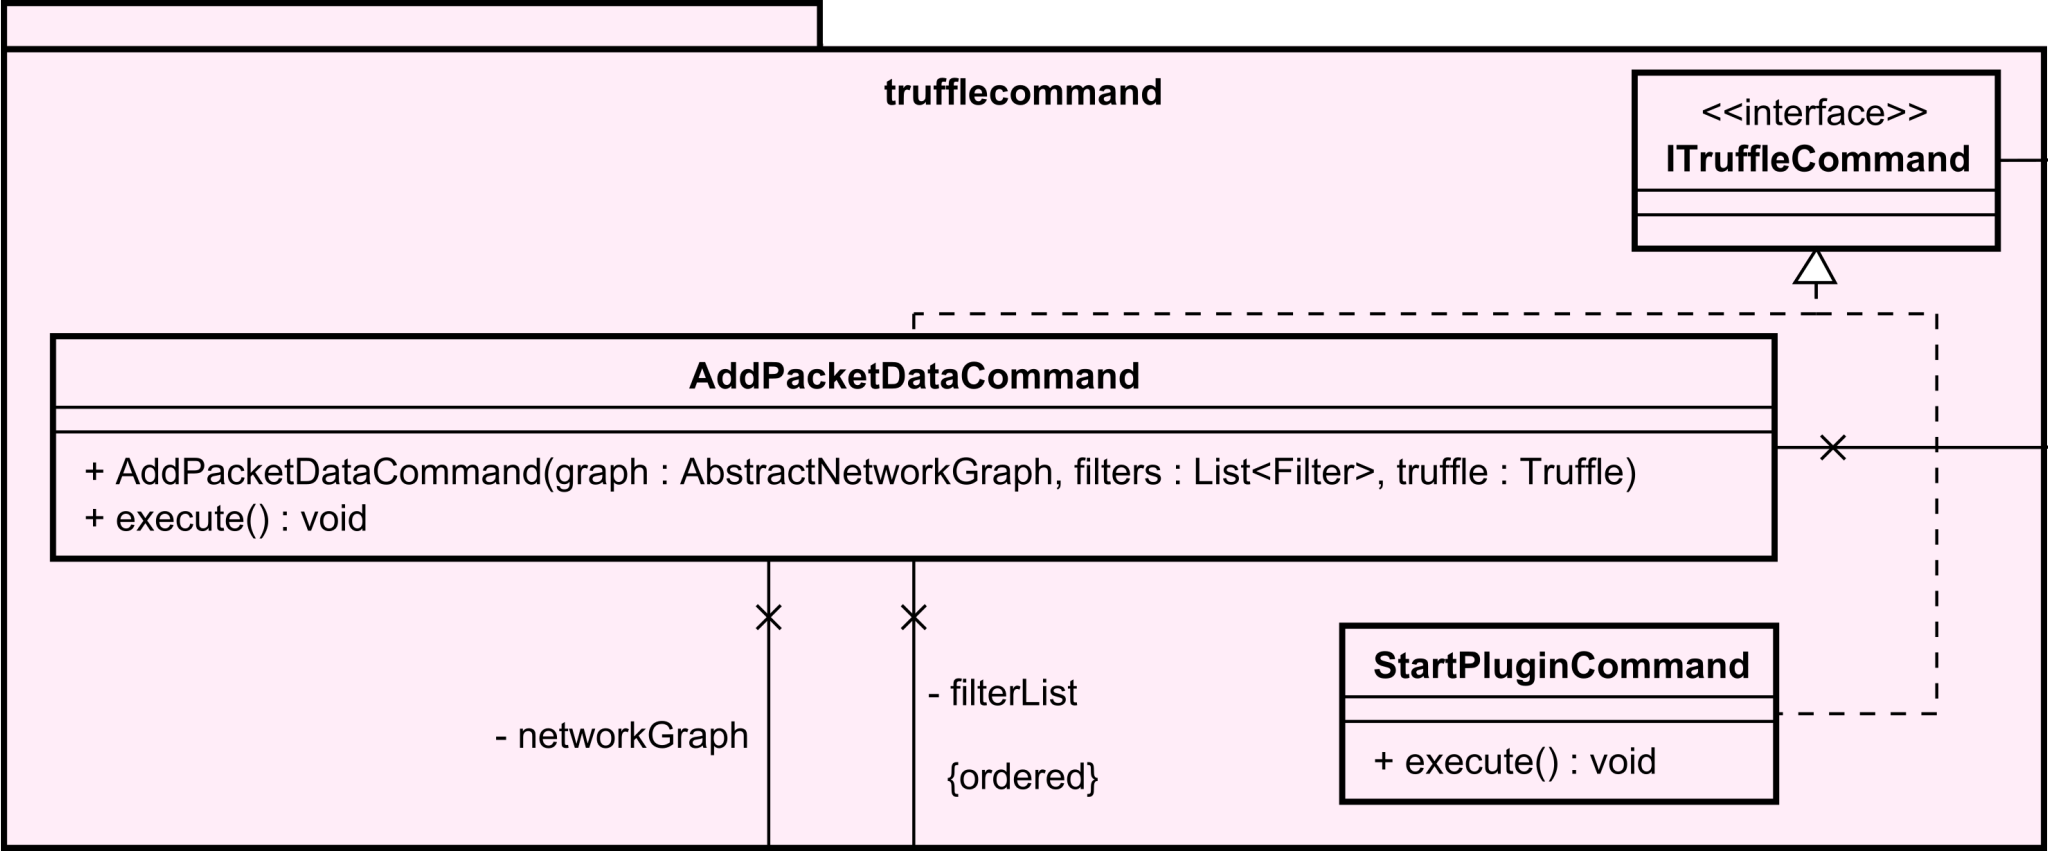
\includegraphics[width=\textwidth]{../diagramimages/trufflecommand.png}
        \caption{trufflecommand-Package}
      \end{figure}

      \medskip
      Jegliche empfangenen Truffles vom \gls{praeprozessor} werden zuerst in Java-Objekt-Truffles umgewandelt, wie
      im \hyperref[subsubsec:truffleprocessor]{truffleprocessor}-Package erklärt. Dort
      werden die erzeugten Java-Truffles in ein Command gesteckt und per \gls{observerpattern}
      wie im \hyperref[subsec:util]{util}-Package beschrieben an alle Interessenten, also die \gls{listener}, verschickt.
      \newline
      \newline
      Es gibt nur einen Command-Typen für die empfangen Truffle-\glspl{paket}, nämlich den
      AddPacketDataCommand. Diese Entscheidung wurde getroffen um das Programm einfach
      zu halten. Commands wie AddNode oder AddEdge sind überflüßig, da diese leicht aus
      dem Inhalt des Truffles gelesen werden können.
      \newline
      \newline
      Der PluginNotRunningCommand wird genau dann vom truffleprocessor verschickt, wenn sich \gls{programname}
      nicht mit \gls{sppname} oder einem äquivalenten Plugin verbinden konnte. Wir
      haben die Funktionalität, dass \gls{programname} automatisch \gls{sppname} startet,
      aufgegeben um die beiden Programme unabhängiger zu gestallten und um dem Benutzter
      mehr Freiheit, beispielsweise bei der \gls{praeprozessor}enwahl, zu geben.

      \subsubsection{usercommand}
      \label{subsubsec:usercommand}

      \begin{figure}[H]
        \centering
        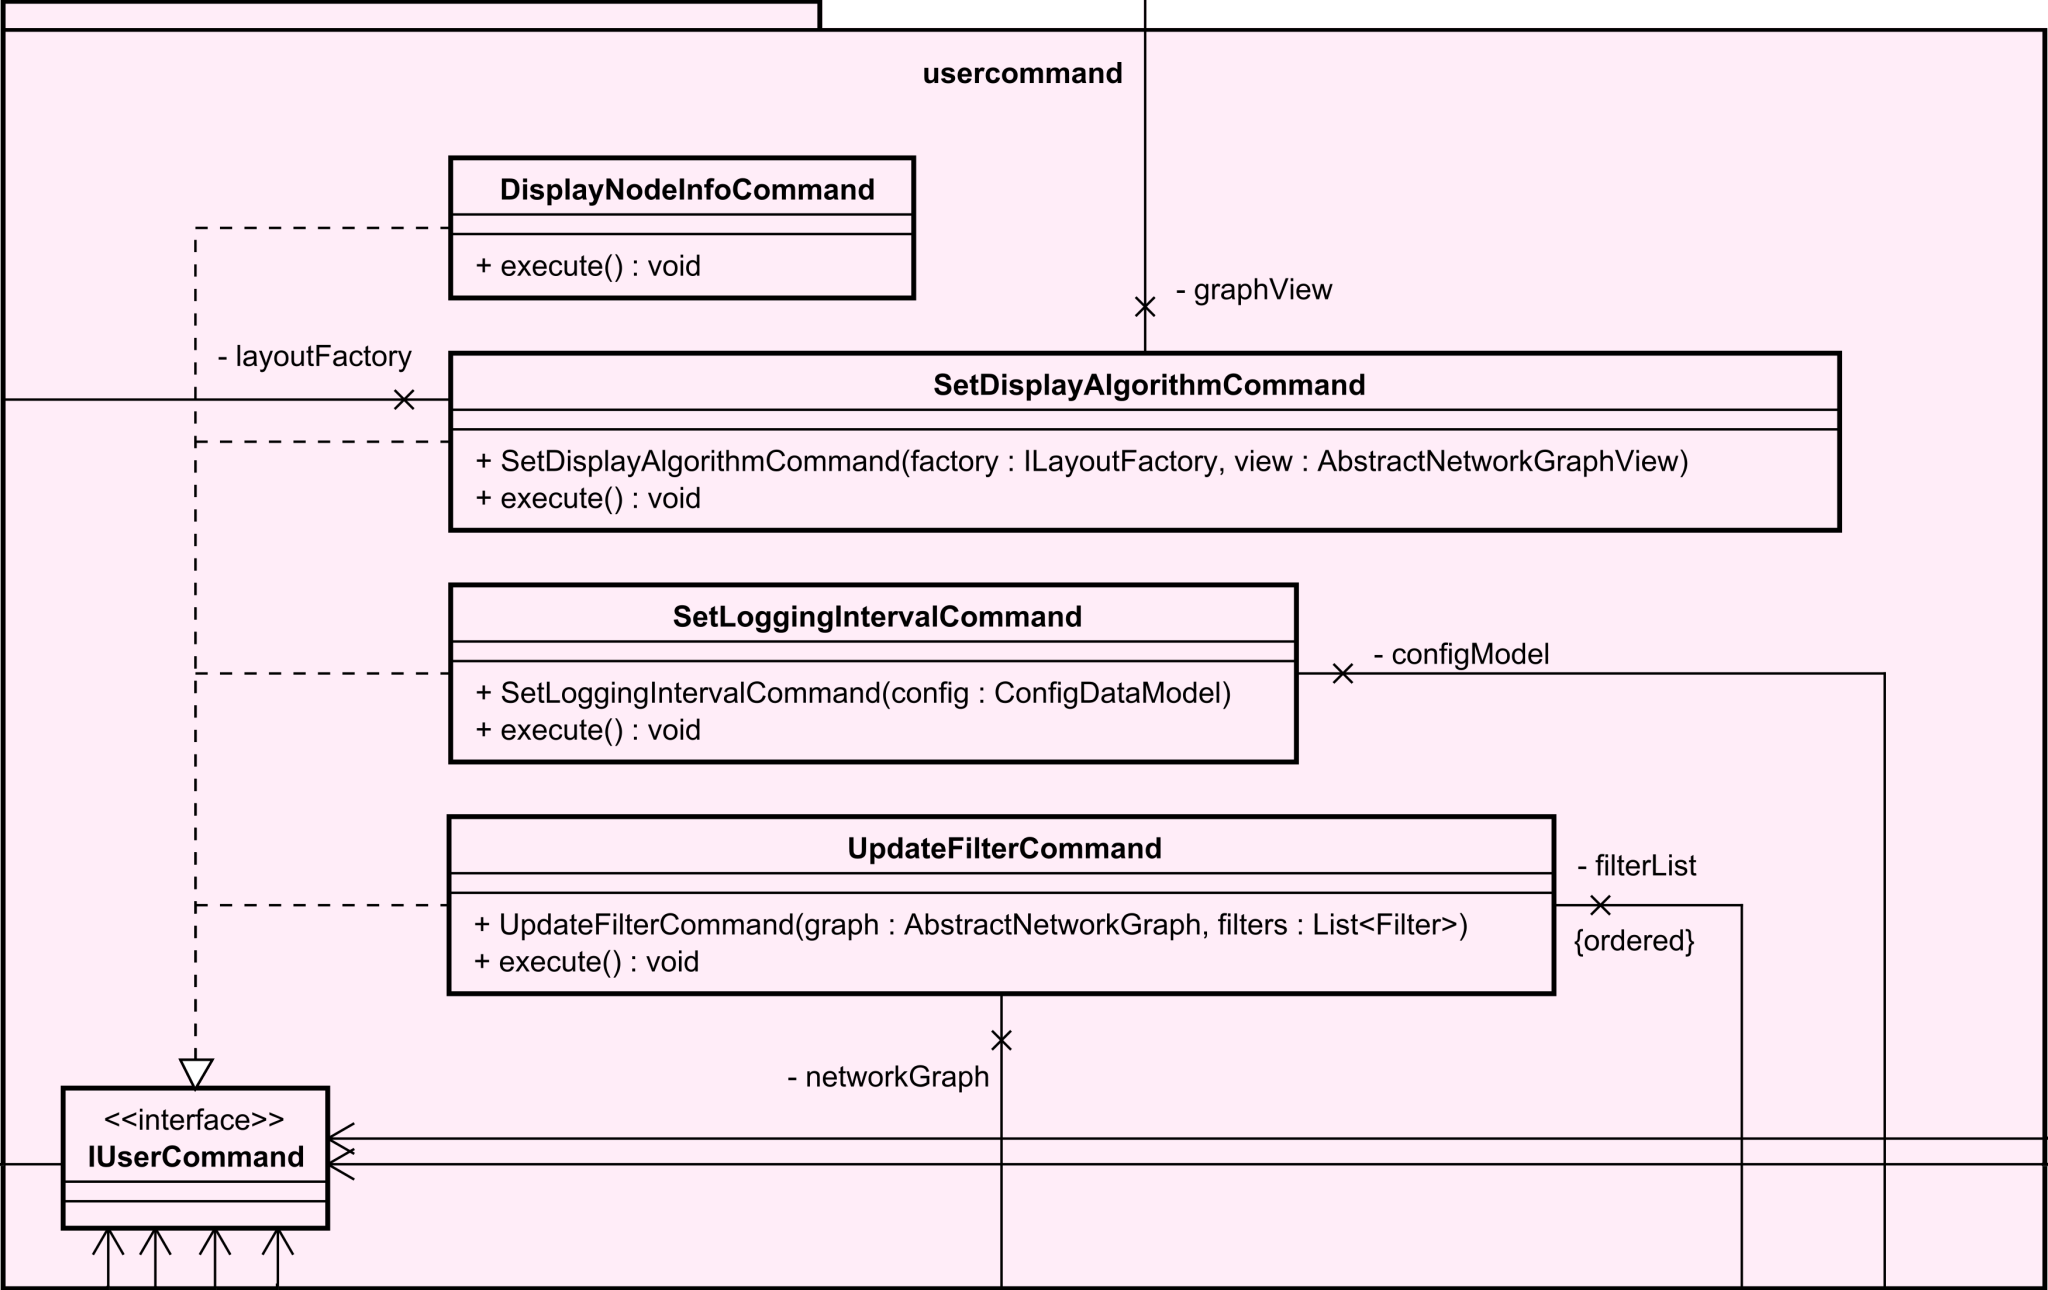
\includegraphics[width=\textwidth]{../diagramimages/usercommand.png}
        \caption{usercommand-Package}
      \end{figure}

      \medskip
      Wenn der Benutzter eine \gls{gui}-Aktion startet, die das Model beeinflusst,
      wird ein entsprechender Command an alle \gls{listener} durch das \gls{observerpattern}, wie im
      \hyperref[subsec:util]{util}-Package beschrieben, verschickt. Für jede mögliche
      \gls{gui}-Aktion, welche das Model beeinflusst, gibt es einen passenden Command.
      Diese werden in den ViewControllern aus dem \hyperref[subsec:view]{view}-Package, wieder nach \gls{observerpattern},
      an den Executor verschickt.

      \subsubsection{queue}
      \label{subsubsec:queue}

      \begin{figure}[H]
        \centering
        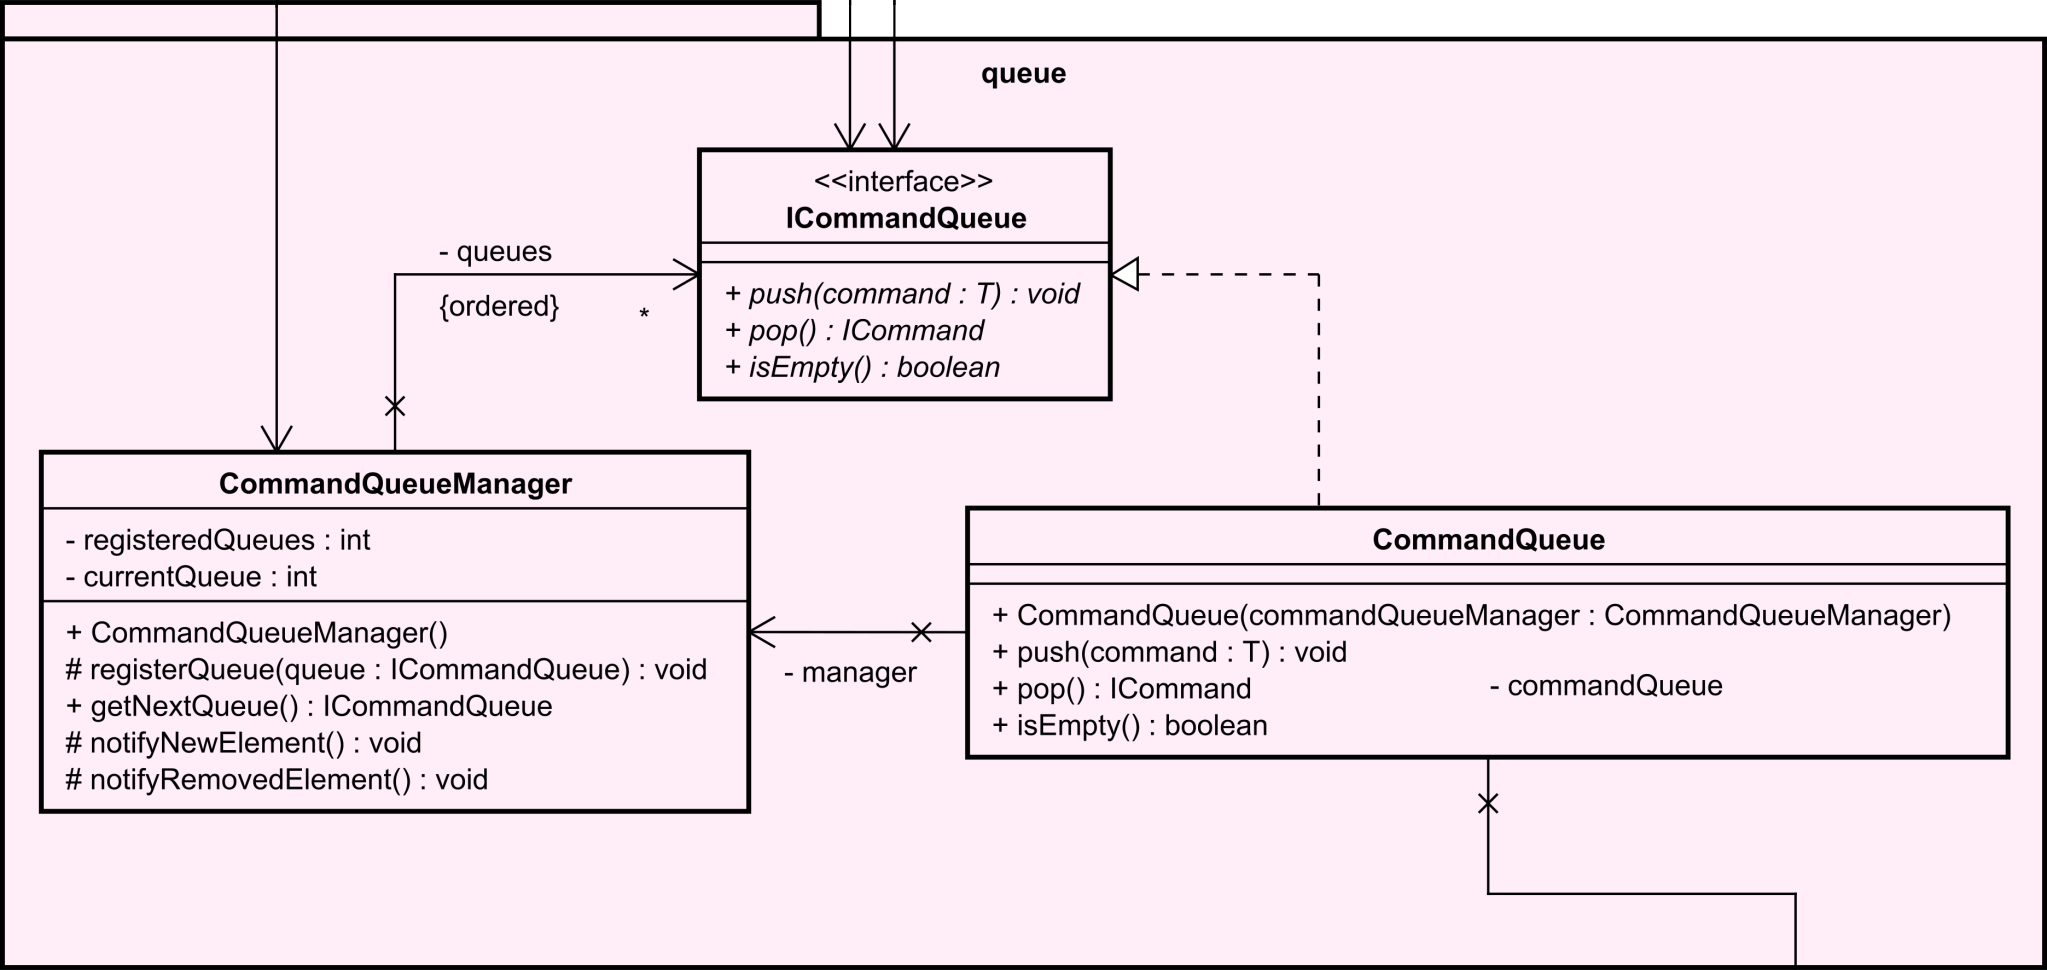
\includegraphics[width=\textwidth]{../diagramimages/queue.png}
        \caption{queue-Package}
      \end{figure}

      \medskip
      Die Commands, welche beispielsweise der Executor abarbeiten soll, werden in
      einer passenden Datenstruktur zwischengespeichert. Es sind ggf. mehrere
      tatsächliche Queues vorhanden, was nach einem Manager verlangt um nach dem
      Round-Robin-Prinzip faire Abarbeitung zu ermöglichen. Diese CommandQueue
      ist das empfangende Ende des \gls{observerpattern} an mehreren Stellen unseres
      Programms. Bei Aktualisierung durch einen \gls{notifier} geht dieser alle
      seine \gls{listener} durch und fügt bei jedem in genau eben diese
      CommandQueue das neue Command-Objekt ein. Die Implementierung der Queues
      als BlockingQueue ermöglicht in diesem Fall die Kommunikation zwischen Threads.